% Chapter 5: RTL Verification
% This file will be included via \input{rtl_verification} in main thesis.tex

\chapter{Functional Verification }
\label{chap:rtl_verification}

% Remove package loading from here - this needs to be in the preamble of thesis.tex
% \usepackage{float}
% \usepackage{placeins}

\section{Register Transfer Level (RTL) Design Verification Strategy}
\label{sec:rtl_verification_strategy}

The verification approach used focused on making the generated RTL design accurately implement the SystemC model while maintaining functional correctness and timing requirement. A complete verification strategy was used to validate the translated design, following industry-standard methods for hardware verification.

\subsection{Testbench Portability and Cross-Platform Verification}
\label{subsec:testbench_portability}

% Use FloatBarrier if placeins is loaded in the preamble, otherwise comment out
% \FloatBarrier

Testbench Portability: This verification strategy uses equivalent test vectors in both SystemC and RTL design simulations for consistent testing across different levels \cite{ref16}. This strategy enables direct comparison of results between the high-level and the synthesised model. The test vectors include a comprehensive set of IEEE 754-compliant floating-point values, covering:
\begin{itemize}
    \item Normal floating-point numbers
    \item Special cases including zero, infinity, and NaN (Not-a-Number) values
    \item Edge cases at the boundaries of the IEEE 754 format
\end{itemize}

\newpage

\begin{figure}[htbp]
    \centering
    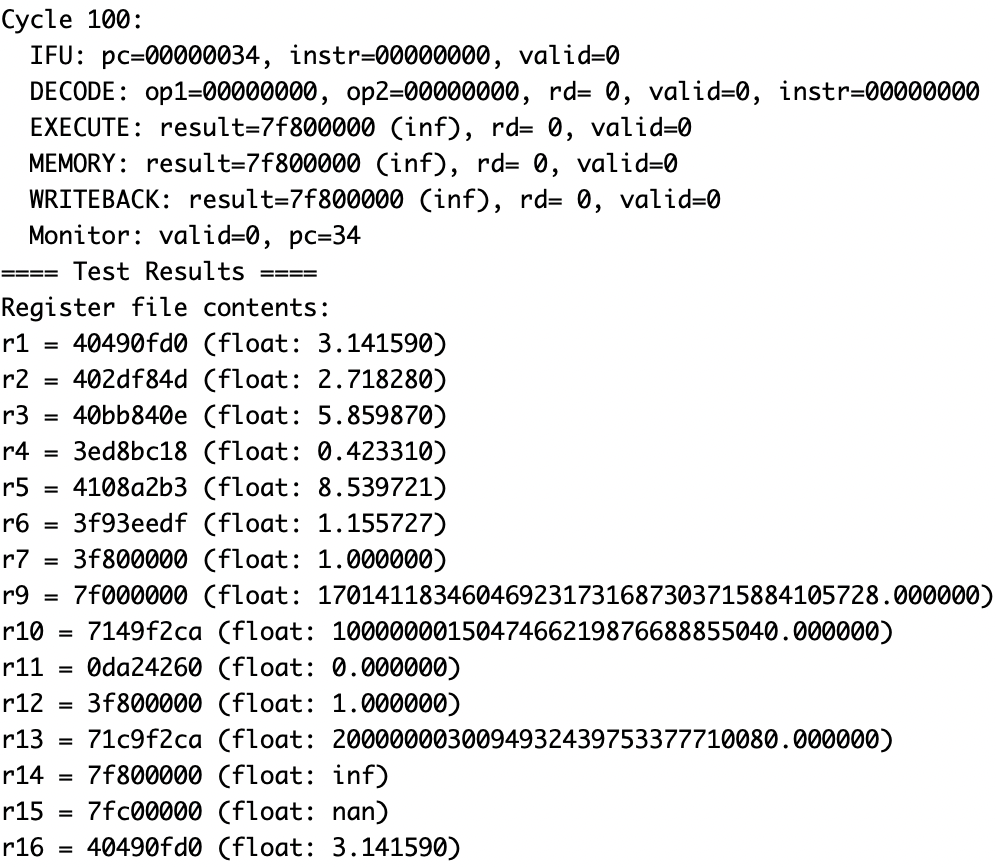
\includegraphics[width=0.95\textwidth]{figures/waveform5.png}
    \caption{Processor state and register content snapshot showing pipeline execution}
    \label{fig:console_output1}
\end{figure}

Figure \ref{fig:console_output1} reveals the floating point processor after cycle 100 with processor storing the outputs in registers after performing IEEE 754 values, including special cases like infinity (r14) and NaN (r15).

\vspace{0.3cm}
\noindent Cross-Verification with RISC-V Spike: The RISC-V ISA simulator Spike serves as a golden reference for cross-verification, ensuring compatibility with the RISC-V floating-point specification (RV32F extension) \cite{ref17}.

\begin{figure}[htbp]
    \centering
    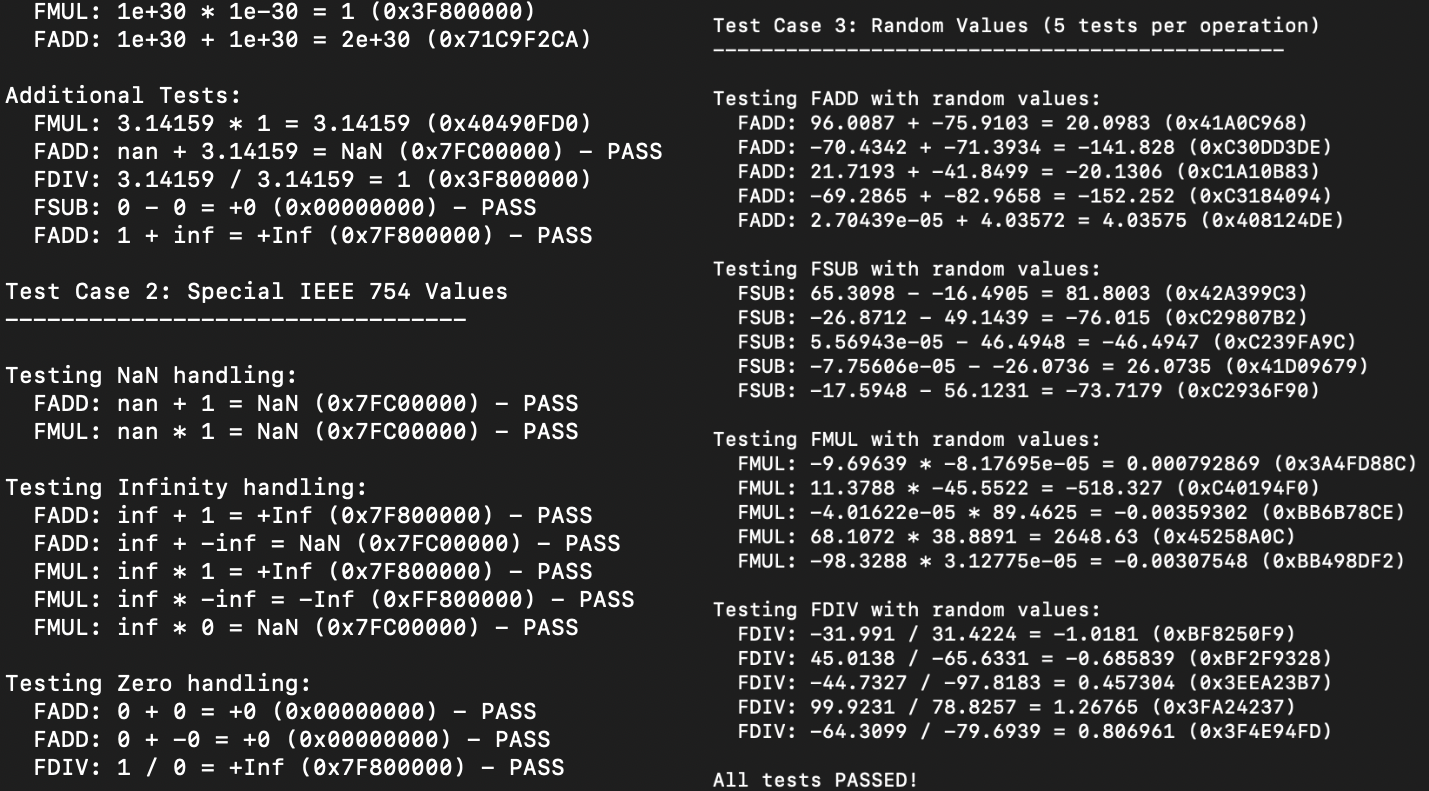
\includegraphics[width=0.95\textwidth]{figures/waveform7.png}
    \caption{Spike cross-verification results for IEEE 754 special cases and random value testing}
    \label{fig:spike_tests}
\end{figure}

\noindent Figure \ref{fig:spike_tests} confirms precise matching between our implementation and the reference model, validating RISC-V RV32F extension compatibility.

\newpage

\subsection{ Waveform Analysis}
\label{subsec:simulation_waveform}
% \FloatBarrier

The waveform analysis is done to confirm timing relationships and data transformations between the SystemC model and the generated RTL. Key verification points include:
\begin{itemize}
    \item Signal propagation delays through the pipeline stages
    \item Data flow integrity from fetch to writeback
    \item Control signal behavior during stall conditions
    \item Floating-point arithmetic unit operation timing
\end{itemize}

The waveform analysis showed us the instruction control behavior and helped in the identifying and solving execution anomalies, in pipeline hazard handling and floating-point exceptions \cite{ref18}.

Comprehensive validation is performed using an extensive set of test cases that include:
\begin{itemize}
    \item Arithmetic operations with various combinations of normal and special values
    \item Edge cases such as overflow, underflow, and precision loss scenarios
    \item Boundary value testing for mantissa and exponent limits
\end{itemize}

\subsection{Waveform Analysis of the Pipelined Floating-Point Processor}
\label{subsec:waveform_analysis}
% \FloatBarrier

The waveforms identified alongside simulation provide critical feedback into the operation of pipelined floating-point processor. Figures \ref{fig:waveform1} through \ref{fig:waveform3} show different waveforms during the simulation of floating-point instructions through the pipeline.

\begin{figure}[htbp]
    \centering
    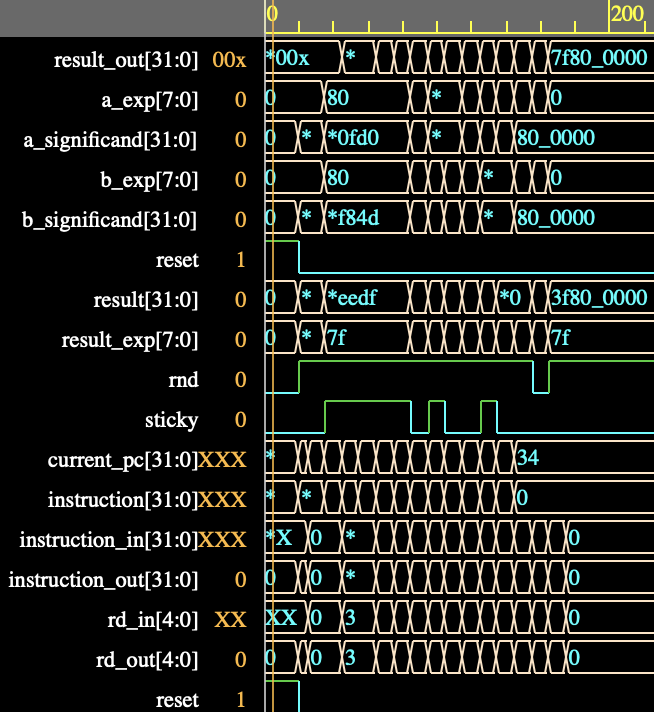
\includegraphics[width=\textwidth]{figures/waveform1.png}
    \caption{Floating-Point Operand and Result Processing Waveform}
    \label{fig:waveform1}
\end{figure}
% \FloatBarrier

Figure \ref{fig:waveform1} displays the core floating-point data path signals during operation. The \textbf{result\_out[31:0]} signal shows the computed IEEE-754 values during execution, including the value \texttt{0x7f80\_0000} which represents infinity and is one of the registers for the test cases for special cases (division by zero).

The decomposition in IEEE 754 calculations is seen through the \textbf{a\_exp[7:0]} and \textbf{a\_significand[31:0]} signals for the first operand, and \textbf{b\_exp[7:0]} and \textbf{b\_significand[31:0]} for the second operand. The displayed values (\texttt{0x0fd0} and \texttt{0xf84d} for the significands) give an idea about the normalized mantissas of floating point operands.

The \textbf{result[31:0]} signal shows the computation output (\texttt{0xeedf} transitioning to \texttt{0x3f80\_0000}, which is 1.0 in IEEE-754). Even the exponent components \textbf{result\_exp[7:0]} with \texttt{0x7f} represent the biased exponent for normalized values. The \textbf{reset} signal initializes the processor, after which normal operation begins. The \textbf{rnd} (rounding mode) and \textbf{sticky} signals show the IEEE-754 rounding logic in action.

% \FloatBarrier
\begin{figure}[htbp]
    \centering
    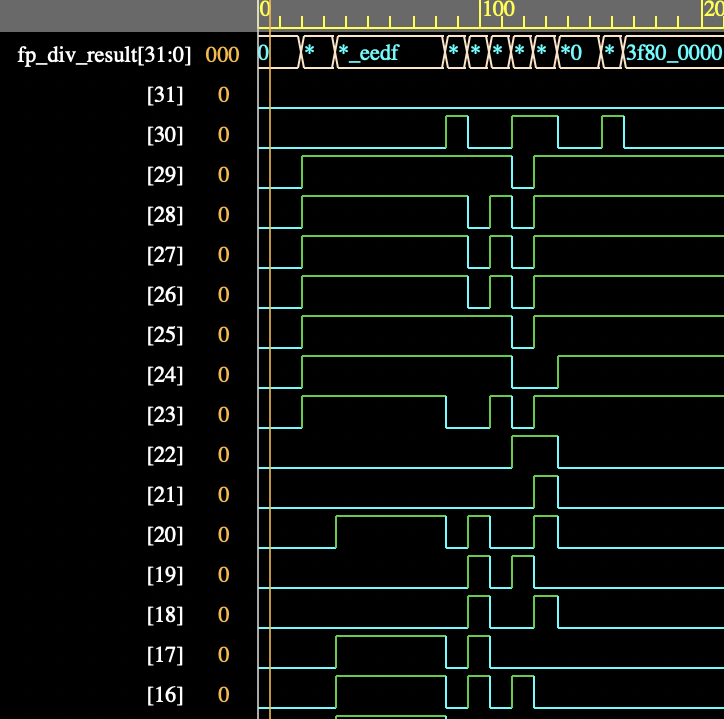
\includegraphics[width=\textwidth]{figures/waveform2.png}
    \caption{Division Unit Signal Analysis Waveform}
    \label{fig:waveform2}
\end{figure}
% \FloatBarrier

Figure \ref{fig:waveform2} gives a proper signal view of the floating-point division unit. The \textbf{fp\_div\_result[31:0]} signal shows the output of the division operation, with the value \texttt{0x3f80\_0000} (1.0) appearing as the result showing the calculation is happening properly.

Each bit signal from \texttt{[31]} through \texttt{[1]} showcase the division algorithm in play. The pattern flow of transitions in these signals emphasises the sequential nature of the division algorithm with shifting and comparison operations.

% \FloatBarrier
\begin{figure}[htbp]
    \centering
    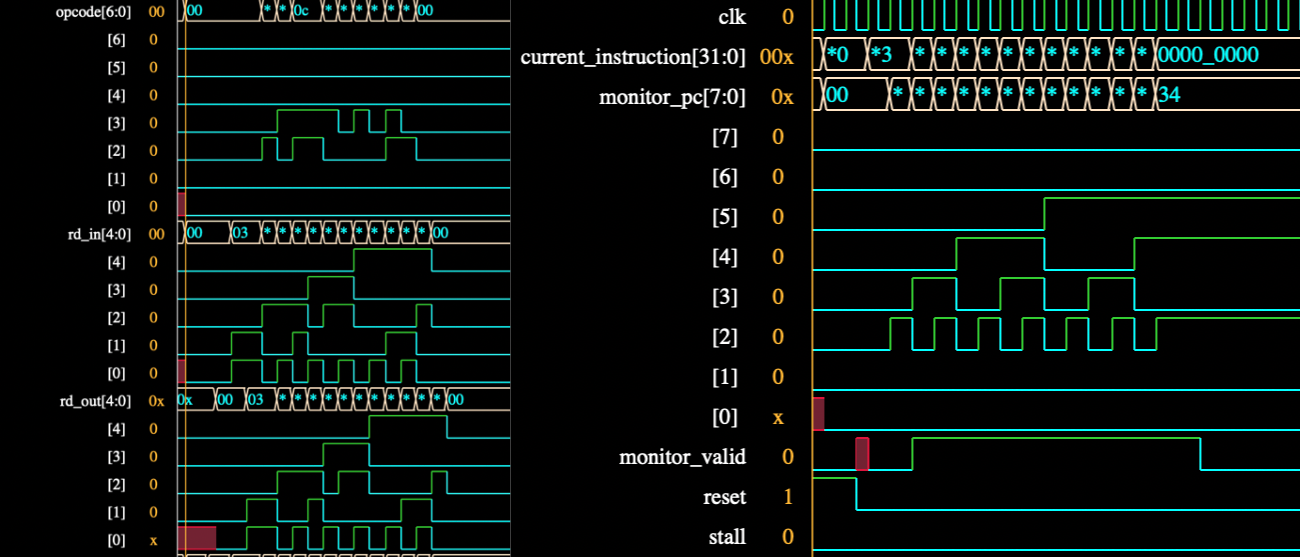
\includegraphics[width=\textwidth]{figures/waveform3.png}
    \caption{Instruction Flow and Operand Handling Waveform}
    \label{fig:waveform3}
\end{figure}
% \FloatBarrier

Figure \ref{fig:waveform3} shows the detailed instruction processing flow. The \textbf{instruction\_in[31:0]}, \textbf{instruction\_out[31:0]}, and \textbf{instruction\_out\_next[31:0]} signals demonstrate the pipelined nature of instruction processing. The staggered transitions in these signals (showing values like \texttt{0x3} for instruction opcodes) confirm proper stage-to-stage handoff through the pipeline.

The \textbf{op1[31:0]} and \textbf{op2[31:0]} signals show operand values (\texttt{0x0fd0} and \texttt{0xf84d}), which are the IEEE-754 components of floating-point values being processed. The \textbf{opcode[6:0]} signal shows the operation type for each instruction, with bits \texttt{[3]} and \texttt{[2]} corresponding to different operations (add, subtract, multiply, divide).

The destination register signals \textbf{rd\_in[4:0]}, \textbf{rd\_out[4:0]}, and \textbf{rd\_out\_next[4:0]} track the register targets for results. The progression of values through these signals shows the sequence of register write destinations, matching the instruction pattern in the testbench.

\section{Verification Results}
\label{sec:verification_results}
% \FloatBarrier

The verification validated proper pipeline functioning with instructions moving through all five stages (Fetch, Decode, Execute, Memory, Writeback) with smooth handling of register file operations and stall conditions. The generated RTL (Register Transfer Level) design preserves the original SystemC architecture code while meeting all timing and functional requirements for FPGA implementation.

\begin{figure}[htbp]
    \centering
     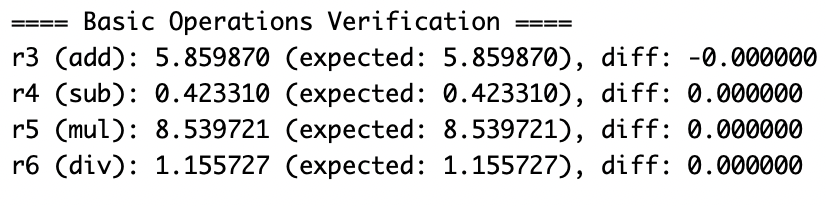
\includegraphics[width=0.95\textwidth]{figures/waveform0.png} 
    \caption{Verification results showing correct execution of basic operations}
    \label{fig:console_output2}
\end{figure}
% \FloatBarrier

Figure \ref{fig:console_output2} and Figure \ref{fig:console_output3} shows verification results for basic operations and special cases, confirming accuracy for standard arithmetic and correct behavior for edge cases, including division by zero producing infinity and proper NaN propagation per IEEE 754 requirements.

\begin{figure}[htbp]
    \centering
     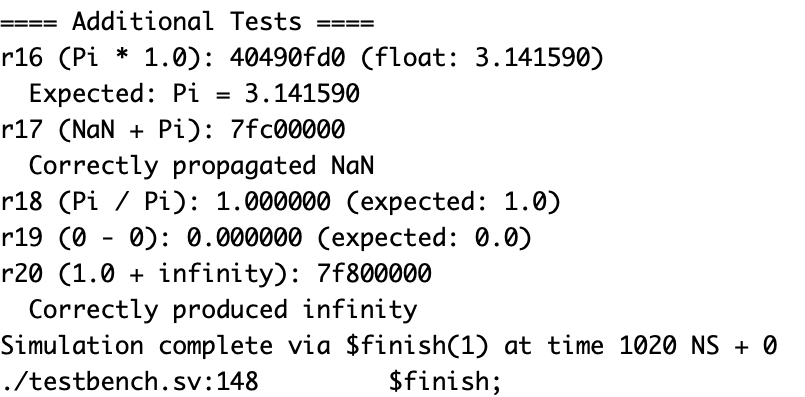
\includegraphics[width=0.95\textwidth]{figures/waveform6.png} 
    \caption{Verification results showing correct execution of special cases handling}
    \label{fig:console_output3}
\end{figure}
% \FloatBarrier

\section{Conclusion}
\label{sec:verification_conclusion}
% \FloatBarrier

The waveforms analysis ensures that the floating-point pipelined processor correctly implements the IEEE-754 floating-point standard  through multiple pipeline stages while the testbench cases ensured accuracy and precision in calculations. The visible signals in our analysis give an idea about both the parallel processing ability of the pipeline and the sequential steps required for arithmetic operations like floating-point division. The successful verification of the RTL established a solid foundation for the subsequent FPGA implementation phase.